\chapter{Mecánica y soporte físico del proyecto} \label{chap:Mecanica}
\chapterimage{figuras/ImagenesPortada/PortadaMecanica.jpg}
\hrule
\vspace{3mm}

Una vez vistas algunas ideas previas generales que deberá tener el prototipo diseñado este capítulo entra de lleno en la descripción de la solución mecánica obtenida así como una comparación con ideas previas.

\section{Visión general} \label{sec:Mecanica:vision_general}

\begin{figure}[H]
    \centering
    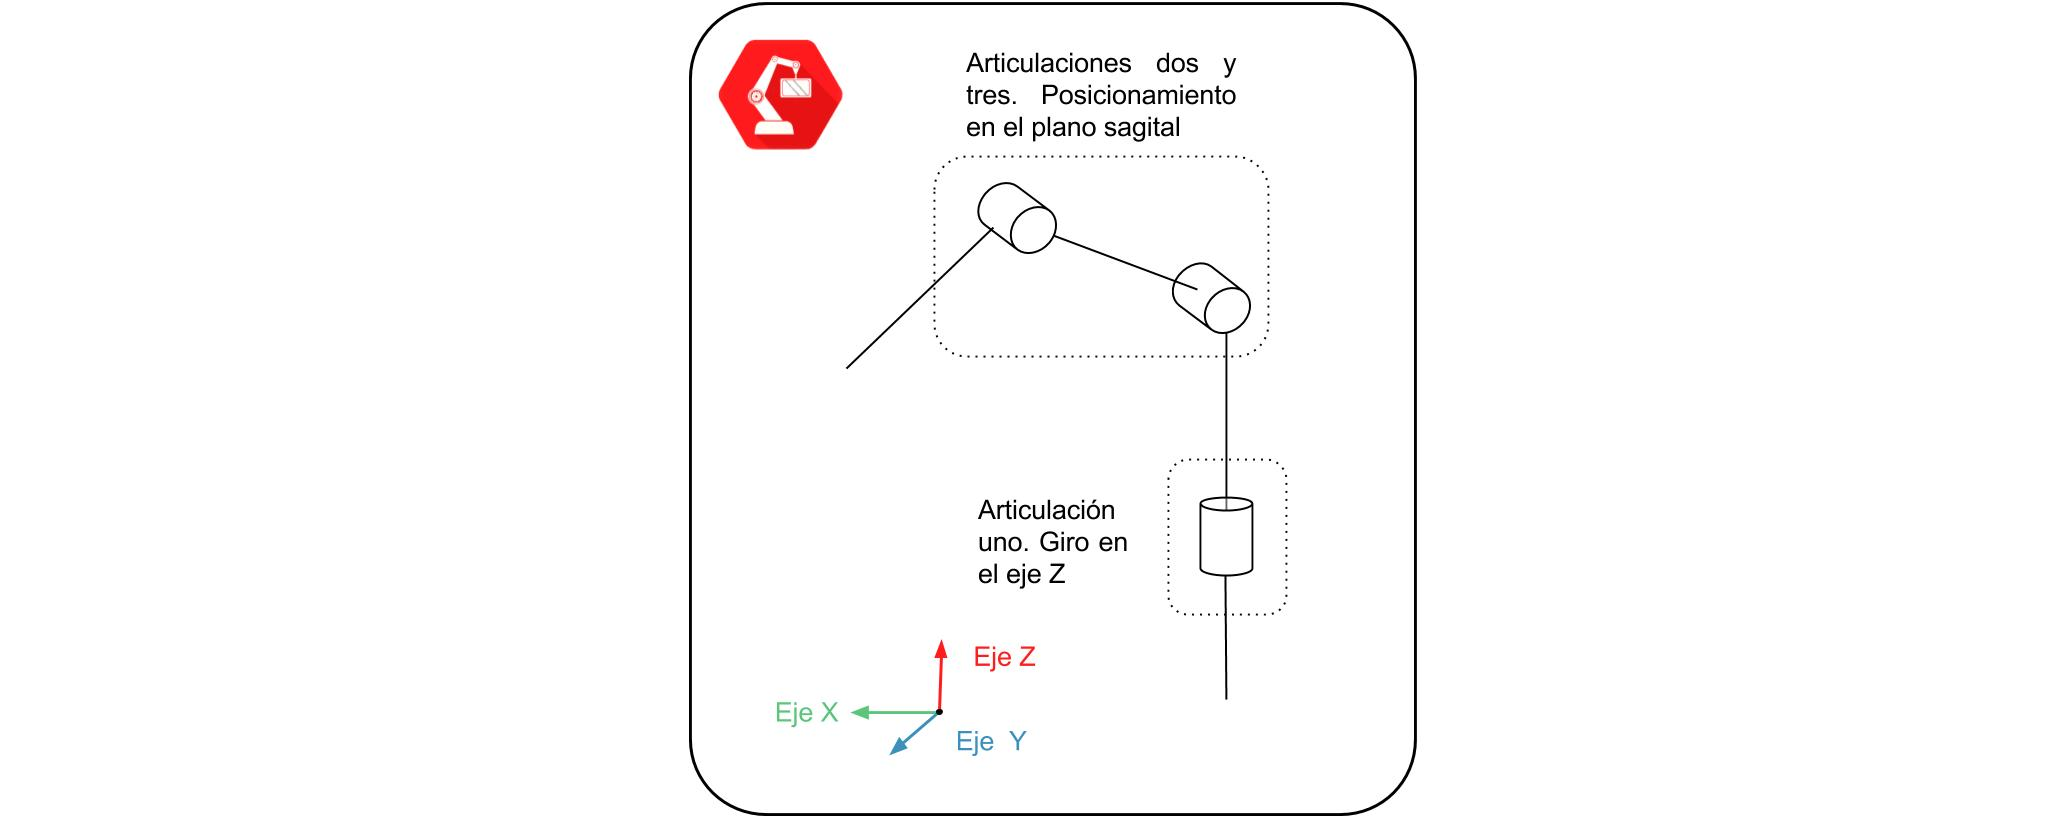
\includegraphics[width=\textwidth]{figuras/Imagenes_Mecanica/modelo_esquematico.jpg}
    \caption{Modelo de los grados de libertad de posición. Convencionalismos tomados}
    \label{fig:Mecanica:convenciones_generales}
    \immagesource{Autor}
\end{figure}

\section{Articulación uno. Giro en el eje Z} \label{sec:Mecanica:articulacion_uno}
    Junto con las articulaciones dos y tres, descritas en la Sección \ref{sec:Mecanica:articulacion_dostres} están consideradas como los grados de libertad que gestionan la posición del extremo del robot en un espacio tridimensional. En adelante se las podrá denominar también "grados de libertad de posición".
    \\

    Esta articulación está actuada por un \ingles{Servo G15 Cube} (descrito en la Sección \ref{sec:Introduccion:materiales_software}. El movimiento de dicho servo se transmite a la articulación a través de un juego de ruedas que, solidarias a la parte superior (parte móvil) de la articulación y por rozamiento, transmiten el movimiento hasta la pista inferior (parte fija a la base del robot).
    \\

    De esta forma aseguramos que el usuario, en cualquier momento, podrá desplazar el robot superando el rozamiento de esta cadena de transmisión anulando, en caso de estar en proceso, el movimiento que pueda estar efectuando el \glosario{servo}.
	\\
	En la figura \ref{fig:Mecanica:giro_z} se puede ver en detalle el montaje de dicha estructura. Las piezas de la imagen se encuentran, con la misma referencia, en el Anexo \ref{app:listadoPiezas}.

	\begin{figure}[H]
		\centering
		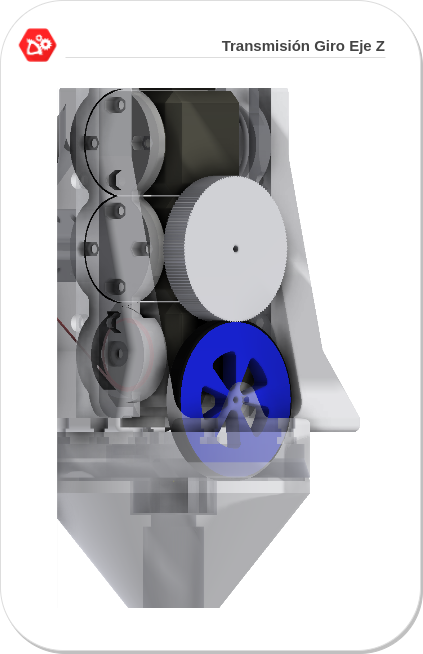
\includegraphics[width=0.5\textwidth]{figuras/Imagenes_Mecanica/RuedasGiroZ.png}
		\caption{Montaje de la transmisión del movimiento del servo a la articulación encargada de girar en Z}
		\label{fig:Mecanica:giro_z}
		\immagesource{Autor}
	\end{figure}

	El apoyo del peso en la última versión se hace sobre un rodamiento \completarCon{coaxial? o como se llamaba?} para conseguir un apoyo completo. Previamente se contempló la posibilidad de utilizar ruedas sobre un carril, de forma que se mantenía una estructura similar a la rueda motriz. En este caso tras probar ambas opciones se optó por colocar la rueda motriz en el lado sobre el que cae la carga del brazo al extenderse para maximizar el apoyo. Este aspecto se ha mantenido al integrar el rodamiento, que asegura un mayor apoyo que las ruedas aun reduciendo el diámetro de dicho apoyo (dificultando la distribución de cargas).

	\completarCon{Imagen de las ruedas con las distintas configuraciones de carga y rueda motriz}

	\completarCon{Imagen de como afecta el cambio de diámetro del apoyo}

\section{Articulaciones dos y tres. Posicionamiento en el plano sagital} \label{sec:Mecanica:articulacion_dostres}
    Estas dos articulaciones son las encargadas de posicionar el extremo en el plano sagital del robot.
    \\

    \begin{figure}[H]
       	\centering
       	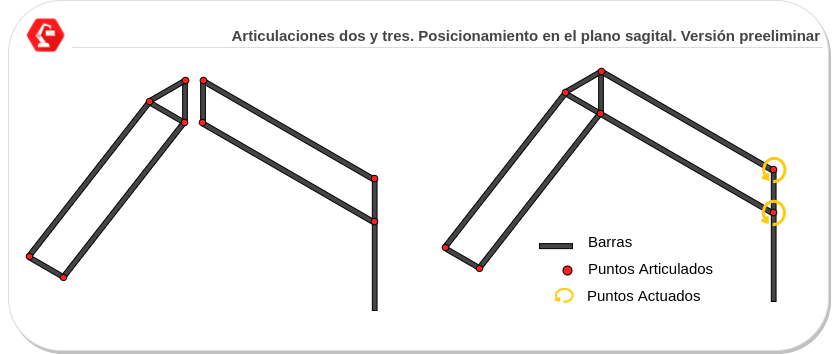
\includegraphics[width=0.9\textwidth]{figuras/Imagenes_Mecanica/mecanismos_4_barras_triangulo.png}
       	\caption{Esquema de la cadena cinemática correspondiente a los \completarCon{Glosario a GDL} dos y tres. Idea preliminar}
       	\label{fig:Mecanica:4_bar_mecanism_triangle}
       	\immagesource{Autor}
    \end{figure}

    Están formadas por dos mecanismos de cuatro barras acoplados en serie. Tienen la particularidad de que las barras son iguales dos a dos, de forma que las barras se mantienen siempre en paralelo.
    \\

    \begin{figure}[H]
    	\centering
    	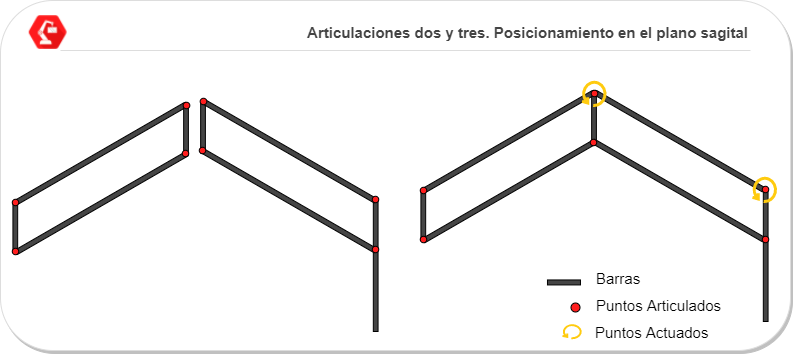
\includegraphics[width=0.9\textwidth]{figuras/Imagenes_Mecanica/mecanismos_4_barras.png}
    	\caption{Esquema de la cadena cinemática correspondiente a los \completarCon{Glosario a GDL} dos y tres}
    	\label{fig:Mecanica:4_bar_mecanism}
    	\immagesource{Autor}
    \end{figure}

    Como se puede ver en la figura \ref{fig:Mecanica:4_bar_mecanism} y \ref{fig:Mecanica:4_bar_mecanism_triangle} la actuación se realiza sobre cada articulación en los puntos marcados. El movimiento se transmite desde los servos ubicados en la base de la articulación 1 hasta las mismas a través de un hilo de \ingles{kevlar}. Un sistema de poleas amplifica y redirige el par hasta los mismos. En la figura \ref{fig:Mecanica:transmision_poleas_cuerda} se puede ver como se redirecciona el hilo desde la base en dirección hacia las articulaciones superiores.

   	\begin{figure}[H]
   		\centering
   		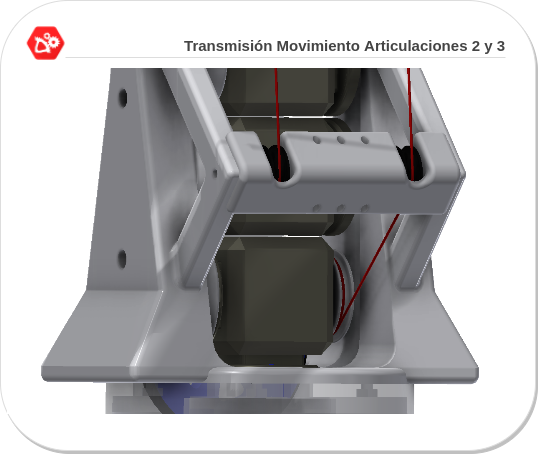
\includegraphics[width=0.6\textwidth]{figuras/Imagenes_Mecanica/TransmisionMotorArticulacion.png}
   		\caption{Montaje de la transmisión del movimiento de los servos a las articulaciones 2 y tres.}
   		\label{fig:Mecanica:transmision_poleas_cuerda}
   		\immagesource{Autor}
   	\end{figure}

   	En las figuras \ref{fig:Mecanica:4_bar_mecanism} y \ref{fig:Mecanica:4_bar_mecanism_triangle} se muestran dos posibles configuraciones mecánicas que se han probado. En la primera, ubicada al principio de la sección (figura \ref{fig:Mecanica:4_bar_mecanism_triangle}) se cuenta con la ventaja de actuar ambas articulaciones sobre el mismo punto de actuación, facilitando la realimentación así como el paso de cables (tanto eléctricos como de transmisión mecánica). Como se puede ver la orientación del extremo depende de los ángulos del triángulo ubicado en el equivalente a la tercera articulación, donde se redirecciona el giro. En este caso las barras a partir de dicho triángulo se encuentran soldadas para hacer la actuación sobre el punto ya mencionado. Otra configuración posible, mostrada en la figura \ref{fig:Mecanica:4_bar_mecanism}, aprovecha esta propiedad de mantener la orientación del extremo a lo largo de la cadena cinemática haciendo que, desde el inicio todas estas conexiones se hagan de forma perpendicular al plano del suelo. De esta forma se puede asegurar que el extremo de dicha cadena mecánica siempre se mantendrá perpendicular al suelo consiguiendo un desacople absoluto de los grados de posición del robot de los grados de libertado que controlan la orientación. En este caso, las barras del extremo no se encuentran soldadas como en el primer caso por lo que el control de la tercera articulación no se puede hacer sobre el mismo punto, como se hacía antes si no que se lleva a la unión de ambos mecanismos. Se ha dado finalmente más peso a la característica de mantener la orientación por facilitar mucho el desarrollo matemático y de control futuros.

\section{Posicionamiento de sensores y actuadores} \label{sec:Mecanica:sensores_actuadore}

	Como e ha anticipado en secciones anteriores los tres motores correspondientes al giro en el eje Z así como el posicionamiento en el plano sagital están ubicados sobre la primera articulación uno encima de otro formando una torre. Desde ahí se dirige a través de hilos el par motor del primer y tercer servo hasta las articulaciones que dos y tres y a través de fricción por ruedas hasta el giro en el eje Z. En la figura \completar se puede ver en detalle dicho montaje así como la fijación a la base de giro.
	\\

	\completarCon{Imagen en detalle de la torre de motores}

	Las articulaciones realimentadas son la articulación dos y la articulación tres, que llevan una realimentación de posición articular a través de un potenciómetro en cada una. El primer grado de libertad, el encargado del giro en el eje Z no está realimentado externamente. En este caso se cuenta con la información proporcionada por el servo y finalmente, la proporcionada por la tablet en el extremo.
	\\

	En el caso de la segunda articulación el potenciómetro se conecta con la propia articulación a través de un juego de engranajes con una relación de \completar que maximiza el uso del potenciómetro, ajustando el rango de movimiento del mismo (\completarCon{cuantos grados gira?}) con el ángulo de giro de la articulación (\completarCon{cuantos grados gira?}). En el caso de la tercera articulación el eje del potenciómetro se encuentra en la misma línea que el eje de giro que se pretende realimentar, el giro es solidario a dicha barra por lo que la relación de giro es unitaria. En la figura \completar se pueden ver ambos montajes: a la derecha la articulación dos con el juego de engranajes; a la izquierda la articulación tres con la transmisión solidaria.

	\completarCon{Añadir fotos de como se enganchan ambos potenciómetros}

\section{Estudio de la cadena cinemática completa} \label{sec:Mecanica:cadena_cinematica}

\completarCon{Hablar de como se reduce la carga hasta los servos: columpios, poleas dobles, palancas, etc}
